%%%%%%%%%%%%%%%%%%%% DRAFT %%%%%%%%%%%%%%
\ifnum\printdraft>0
	\texttt{Some meta text here?}
\else
\begin{center}
	\textbf{--- DRAFT PARTS ---}
\end{center}
\fi
%%%%%%%%%%%%%%%%%%%% END DRAFT %%%%%%%%%%

Main focus of this report is to analyze, and compare between models, the performance impact of varying vocabulary size for different data types as well as difficulties of distinguish the eight different topics. The result of the analysis can be seen in Figure \ref{fig:hitratio} \& \ref{fig:confmat} and Table \ref{tab:similarity}.\\\\
Figure \ref{fig:hitratio} shows, for the different models and data types, the overall hit ratio of correct classification as a function of vocabulary size after $\chi^2$ pruning. Comparing the figures one can establish that the maximum accuracy of 76\% is attained with binary inputs by Multinomial at a vocabulary size of 1022 words.

\onecolumn
\subsection{Hit Ratio}
\newcommand{\figwidth}{0.49\textwidth}
\begin{figure}[H]
	\centering
	\begin{subfigure}[b]{\figwidth}
		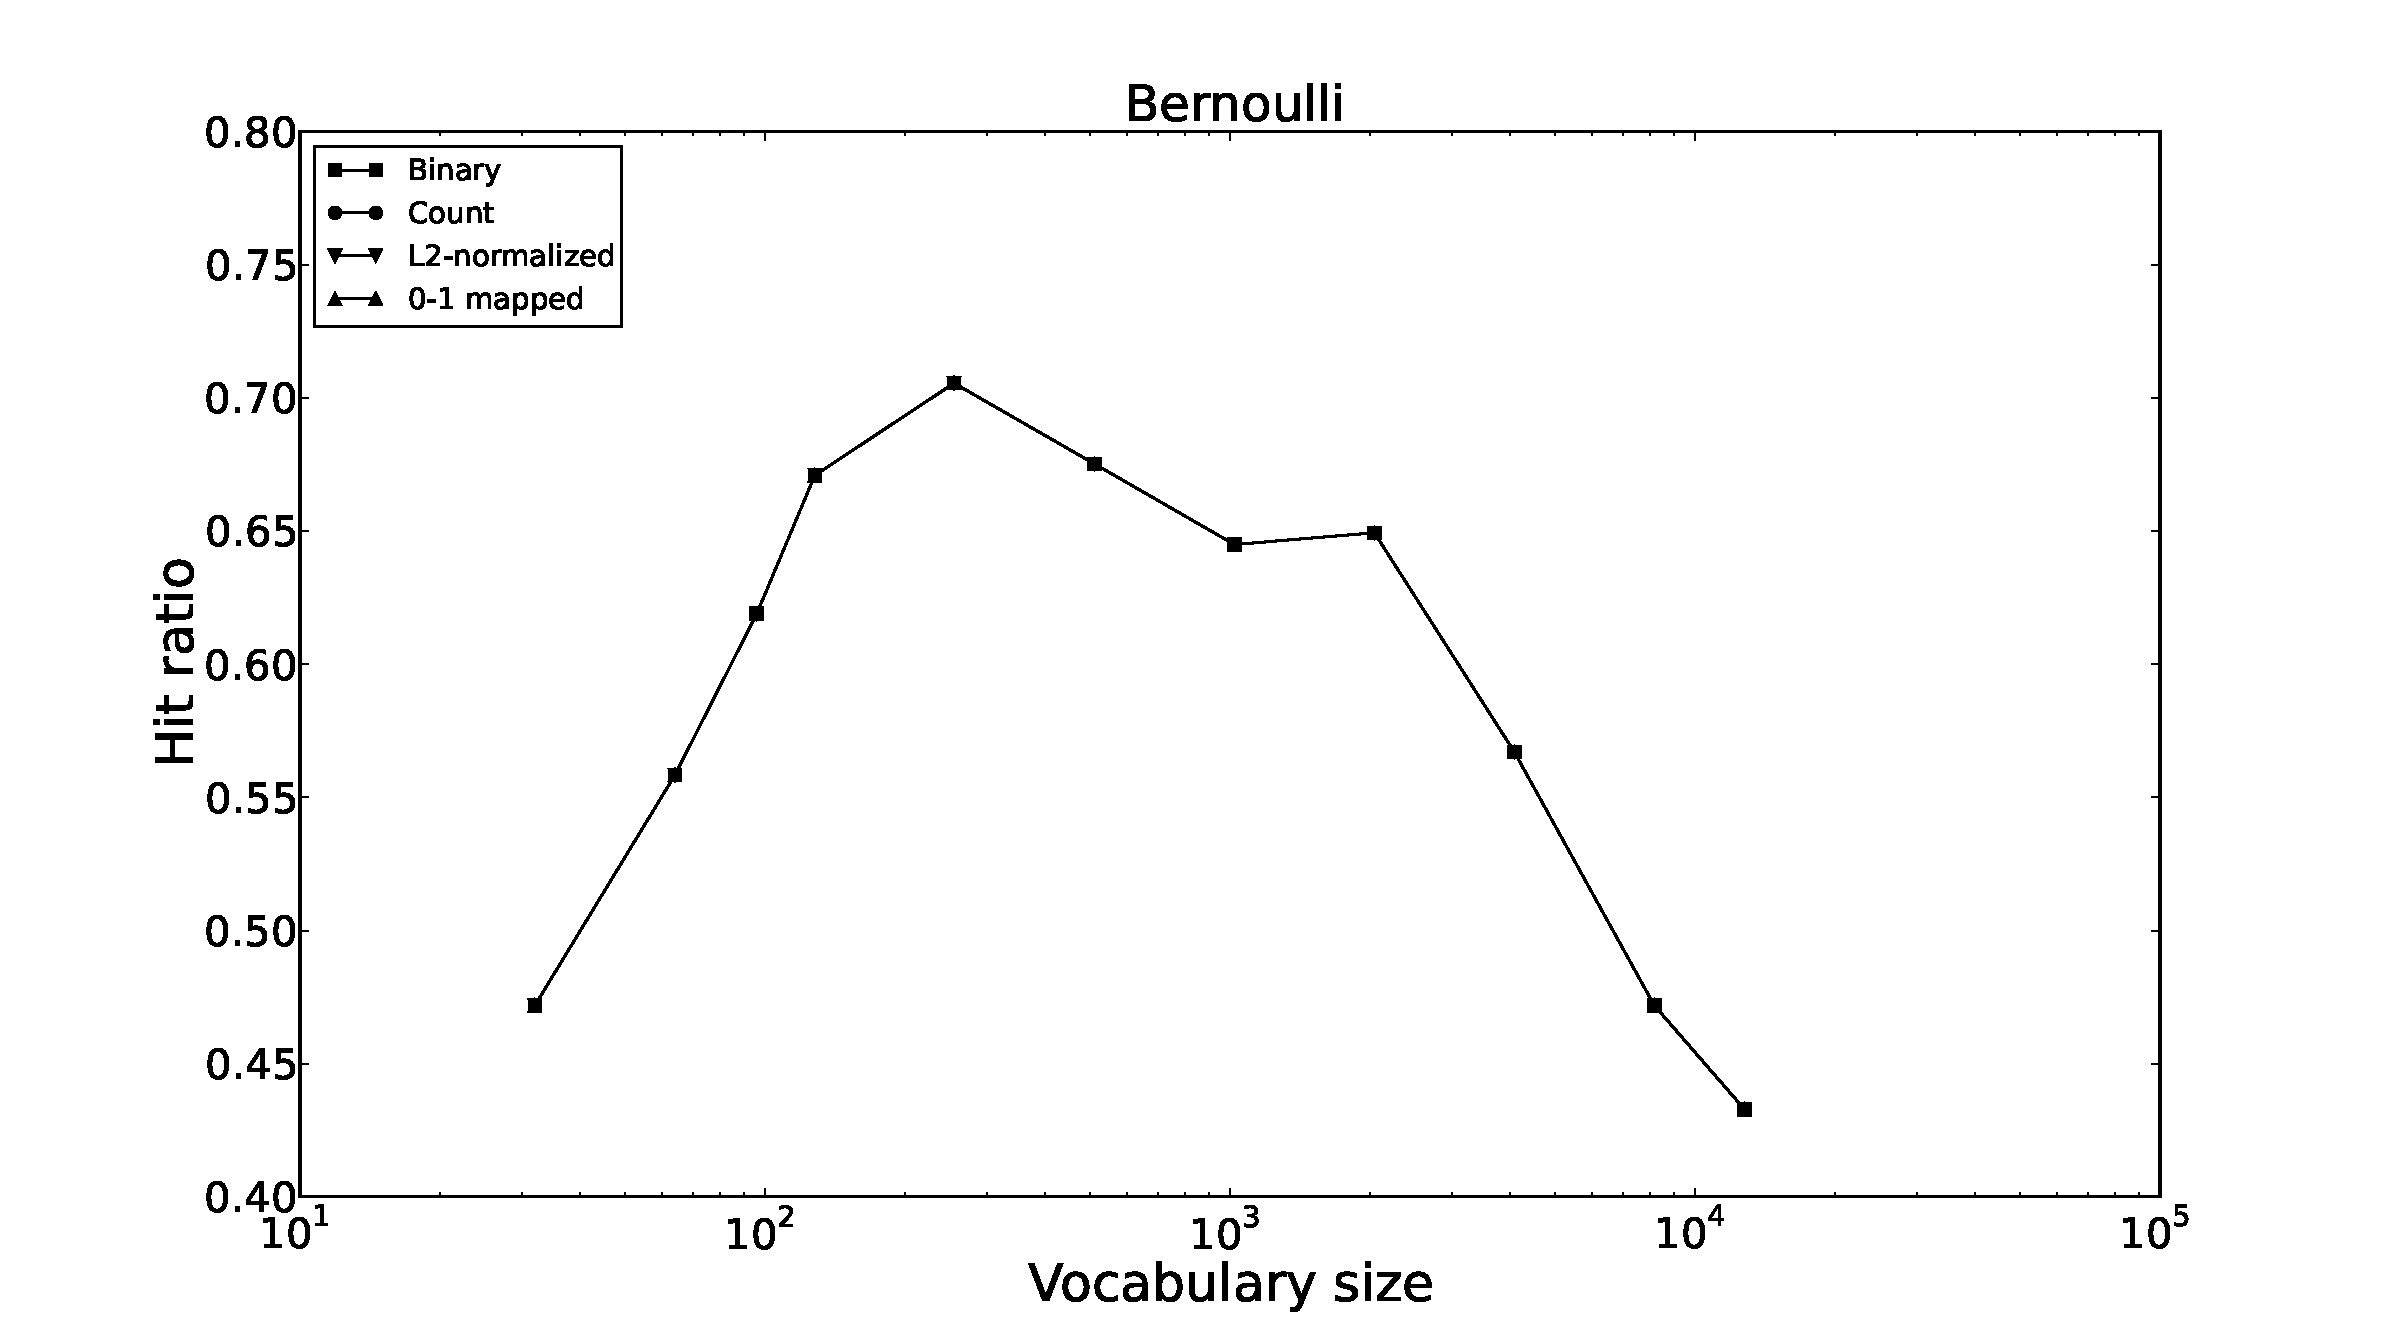
\includegraphics[width=\textwidth]{img/Bernoulli-hitrate-eps-converted-to.pdf}
		\caption{Hit ratio of Bernoulli classifier with varying vocabulary size. All values greater than zero is mapped to one, hence the different data types result in same accuracy.}
		\label{fig:hitratio-nb}
	\end{subfigure}
	~
	\begin{subfigure}[b]{\figwidth}
		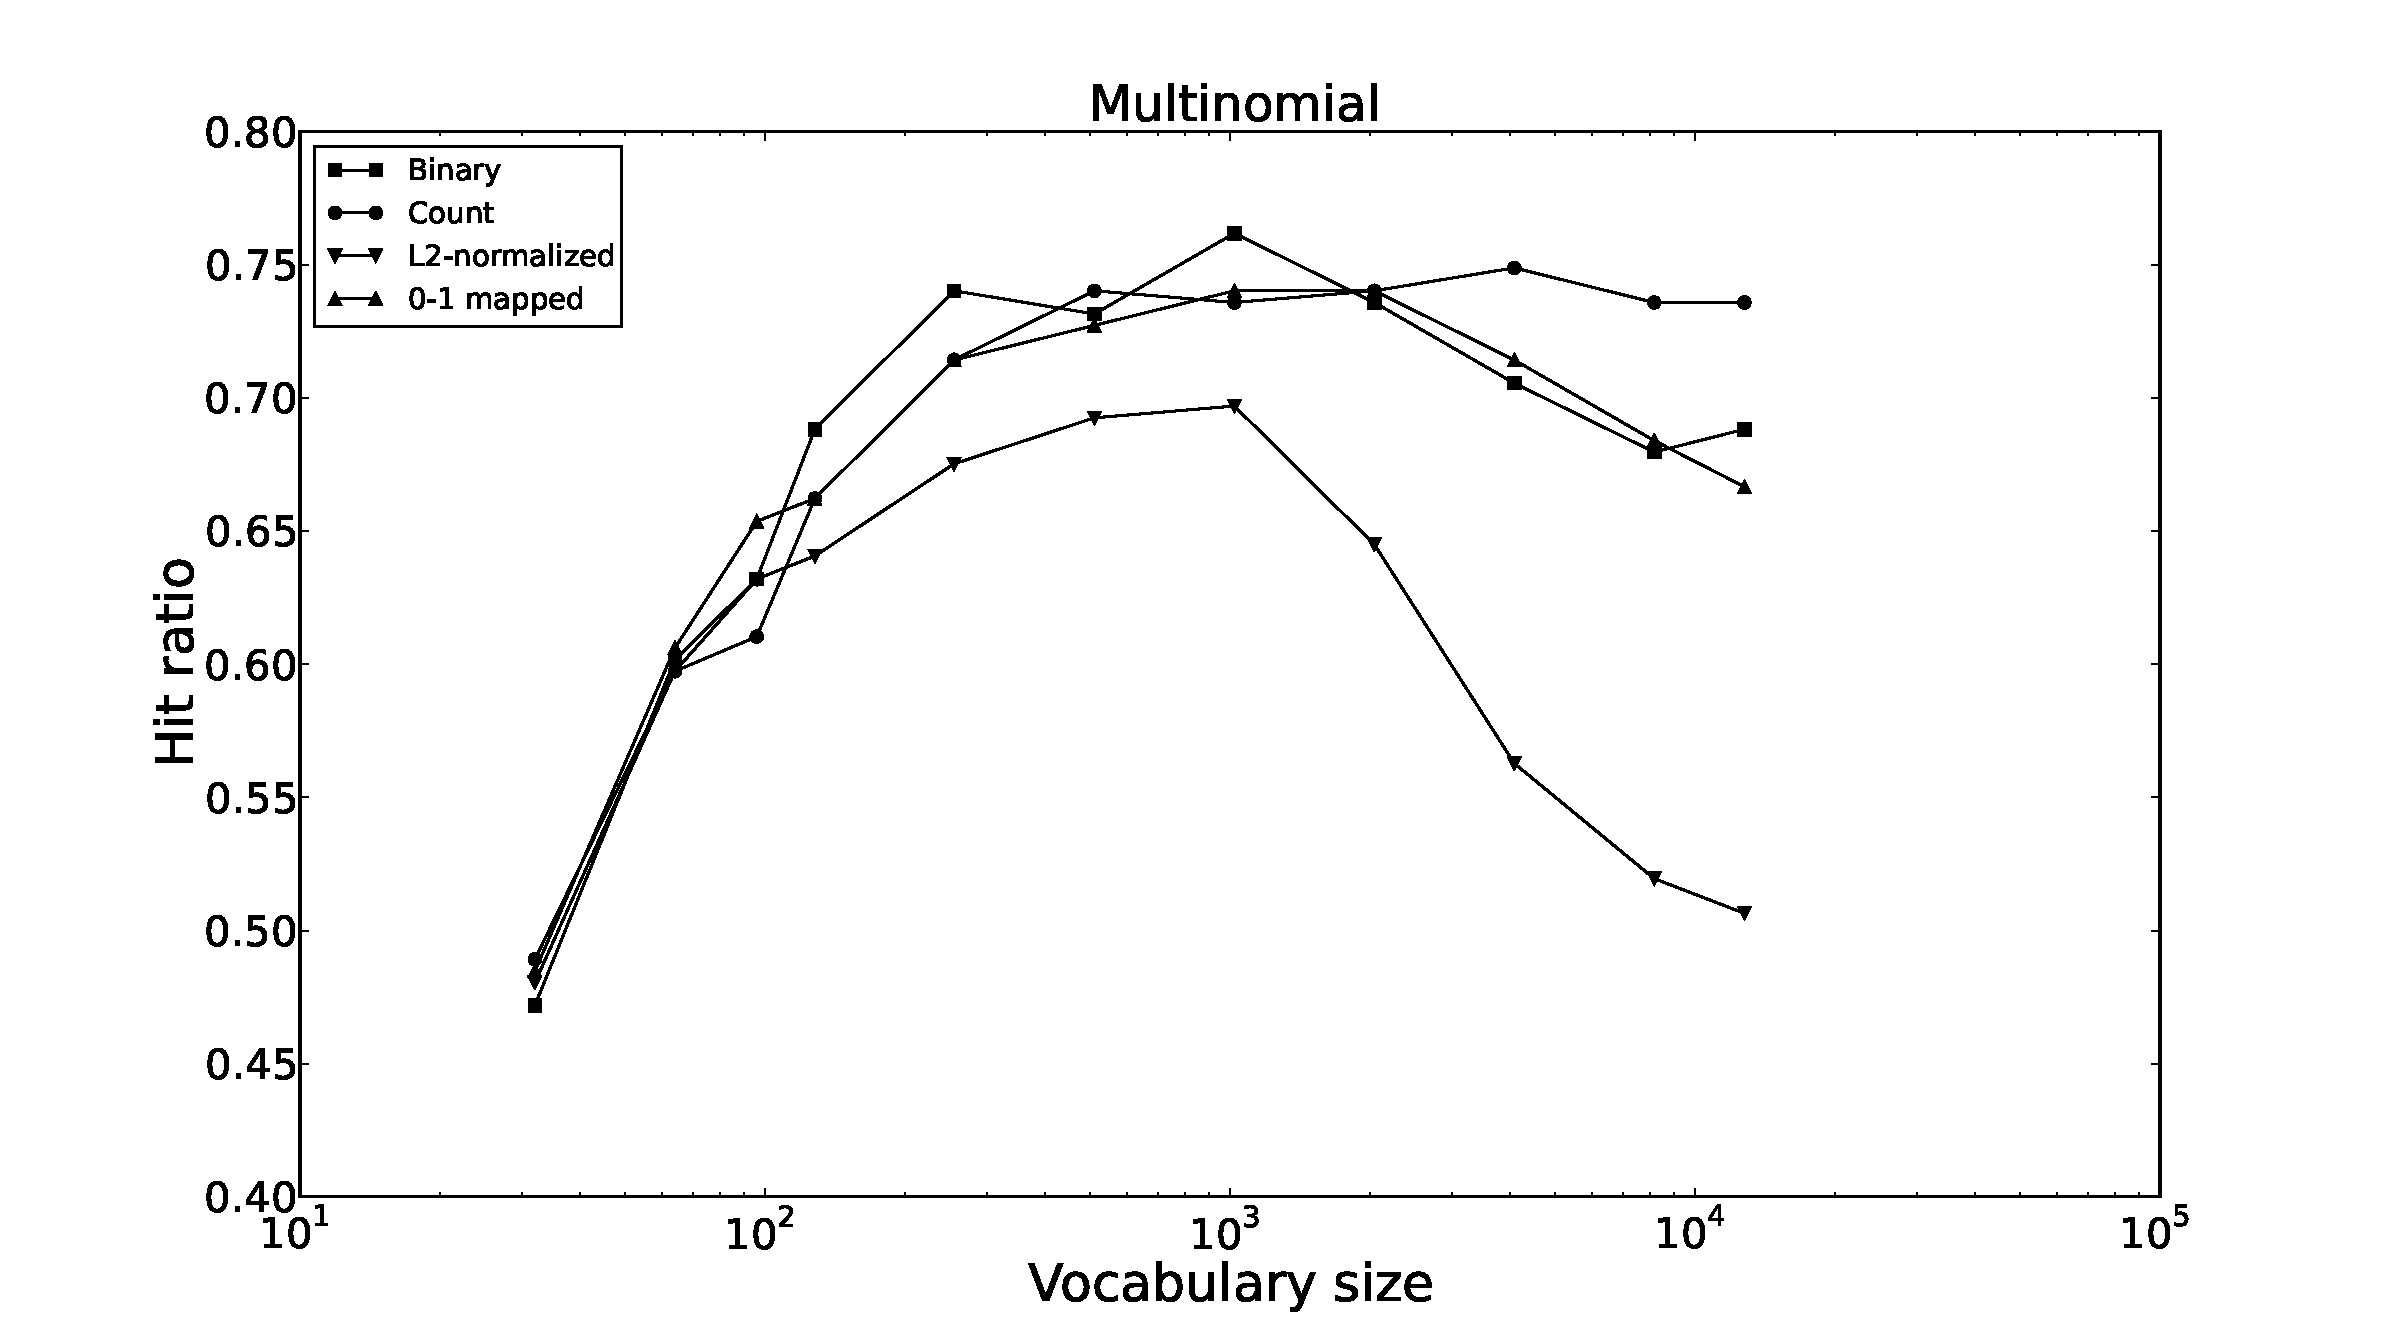
\includegraphics[width=\textwidth]{img/Multinomial-hitrate-eps-converted-to.pdf}
		\caption{Hit ratio of Multinomial classifier with varying vocabulary size.}
		\label{fig:hitratio-mn}
	\end{subfigure}
	\\
	\begin{subfigure}[b]{\figwidth}
		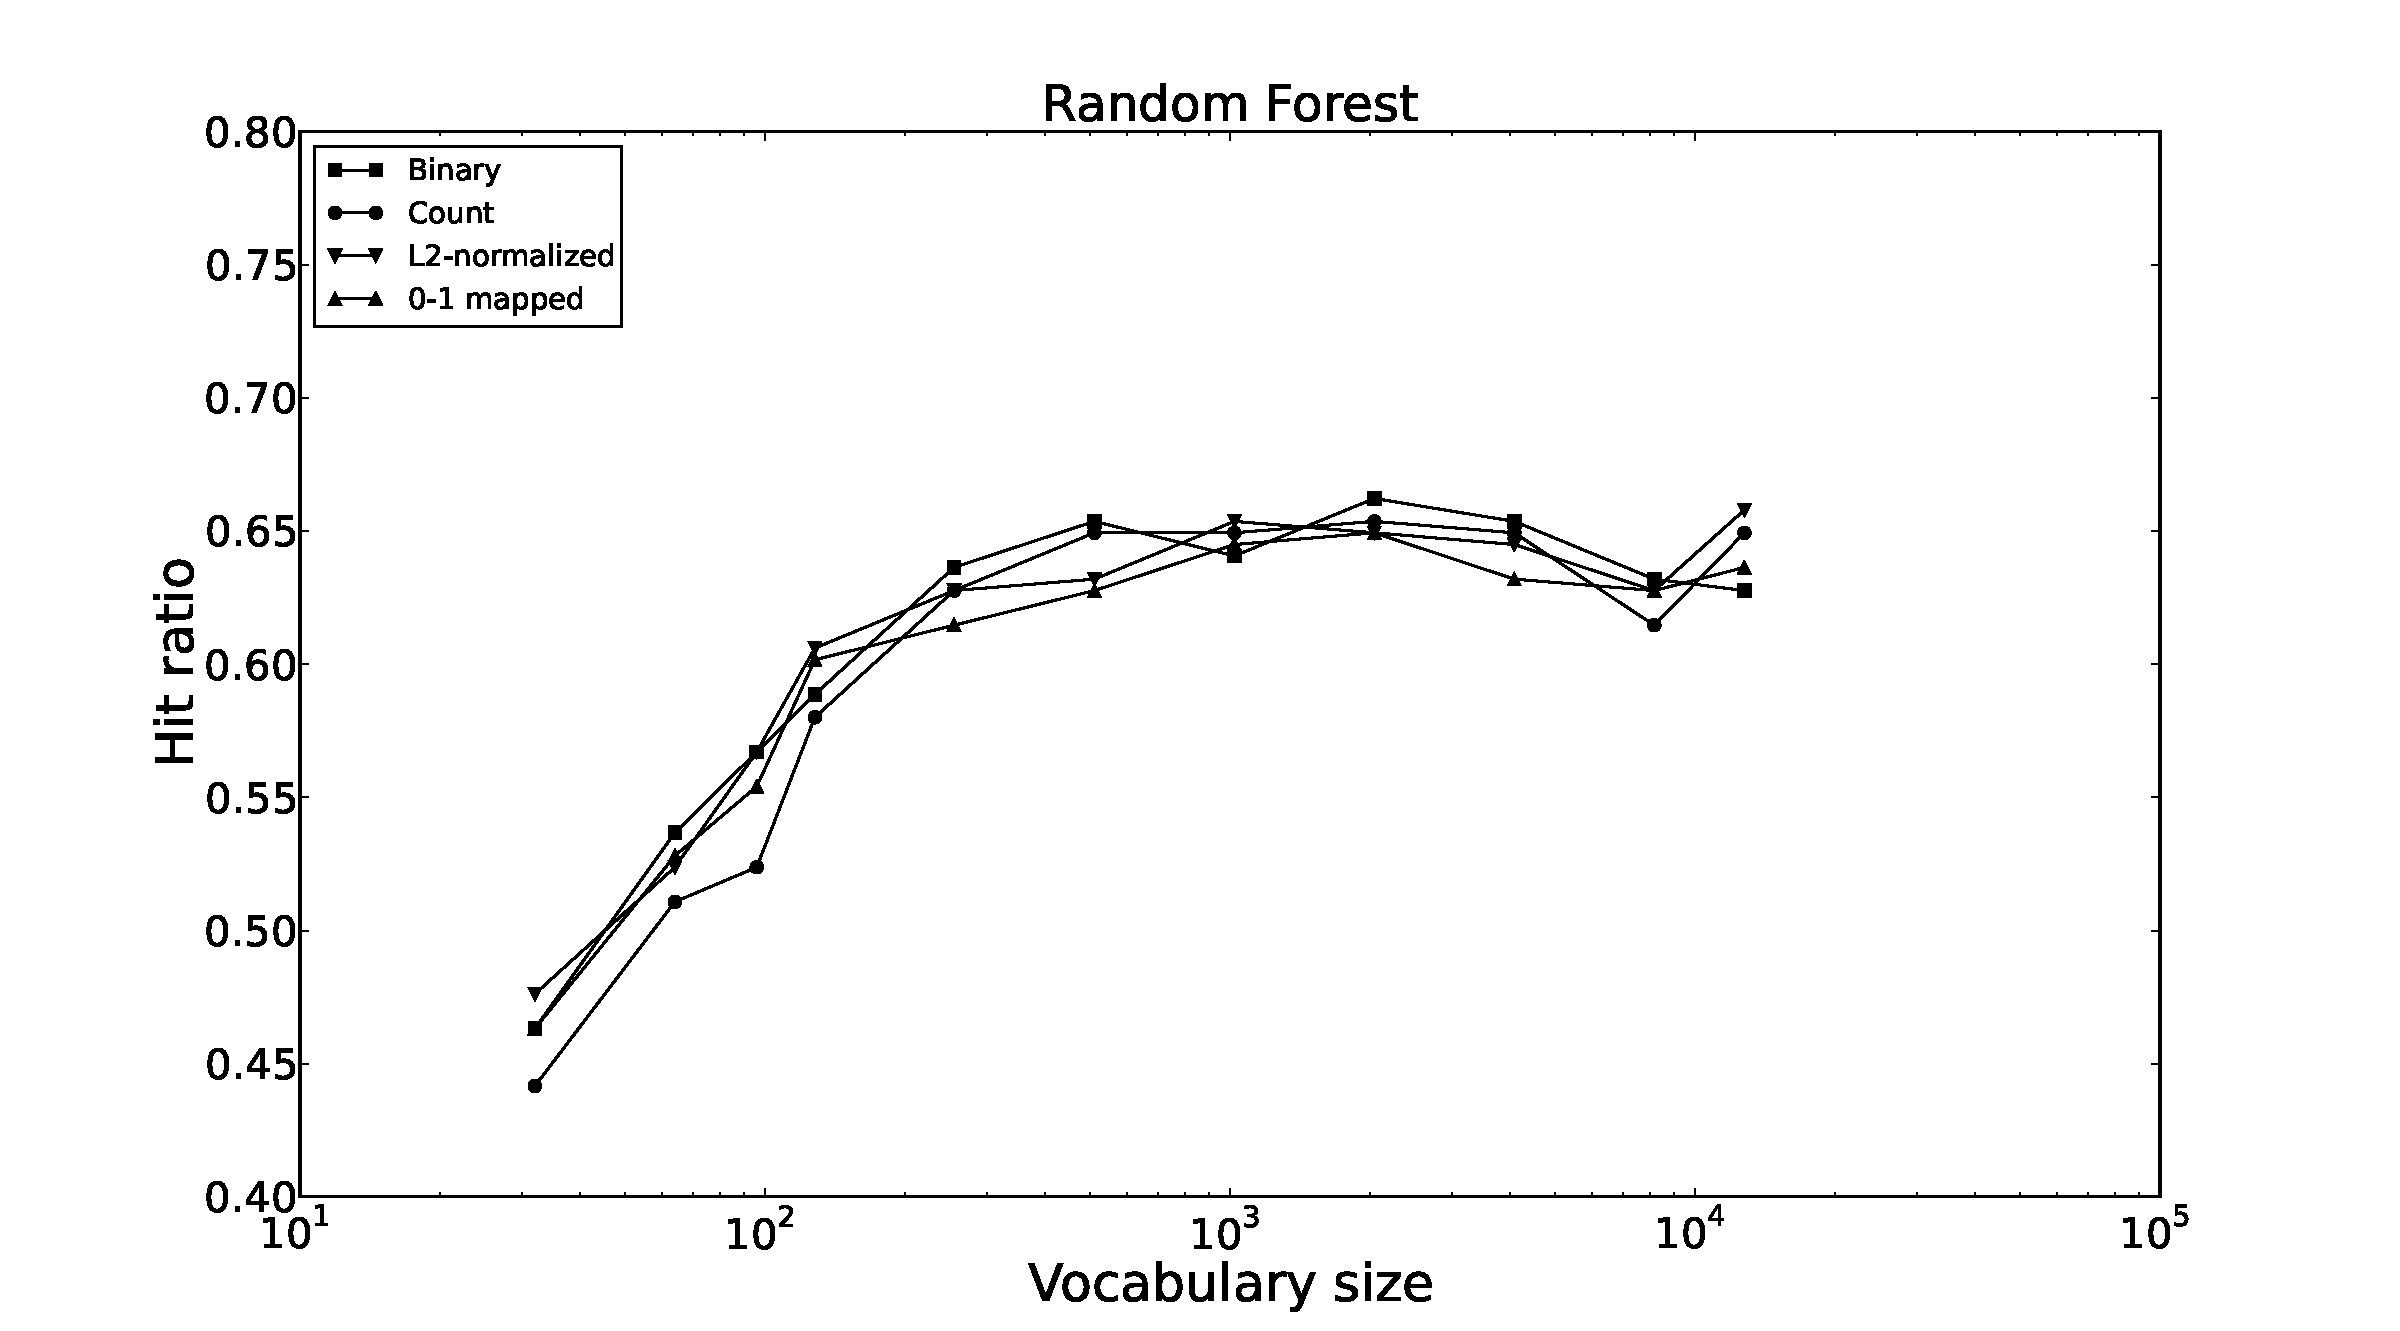
\includegraphics[width=\textwidth]{img/Random-Forest-hitrate-eps-converted-to.pdf}
		\caption{Hit ratio of Random Forest classifier with varying vocabulary size.}
		\label{fig:hitratio-rf}
	\end{subfigure}
	~
	\begin{subfigure}[b]{\figwidth}
		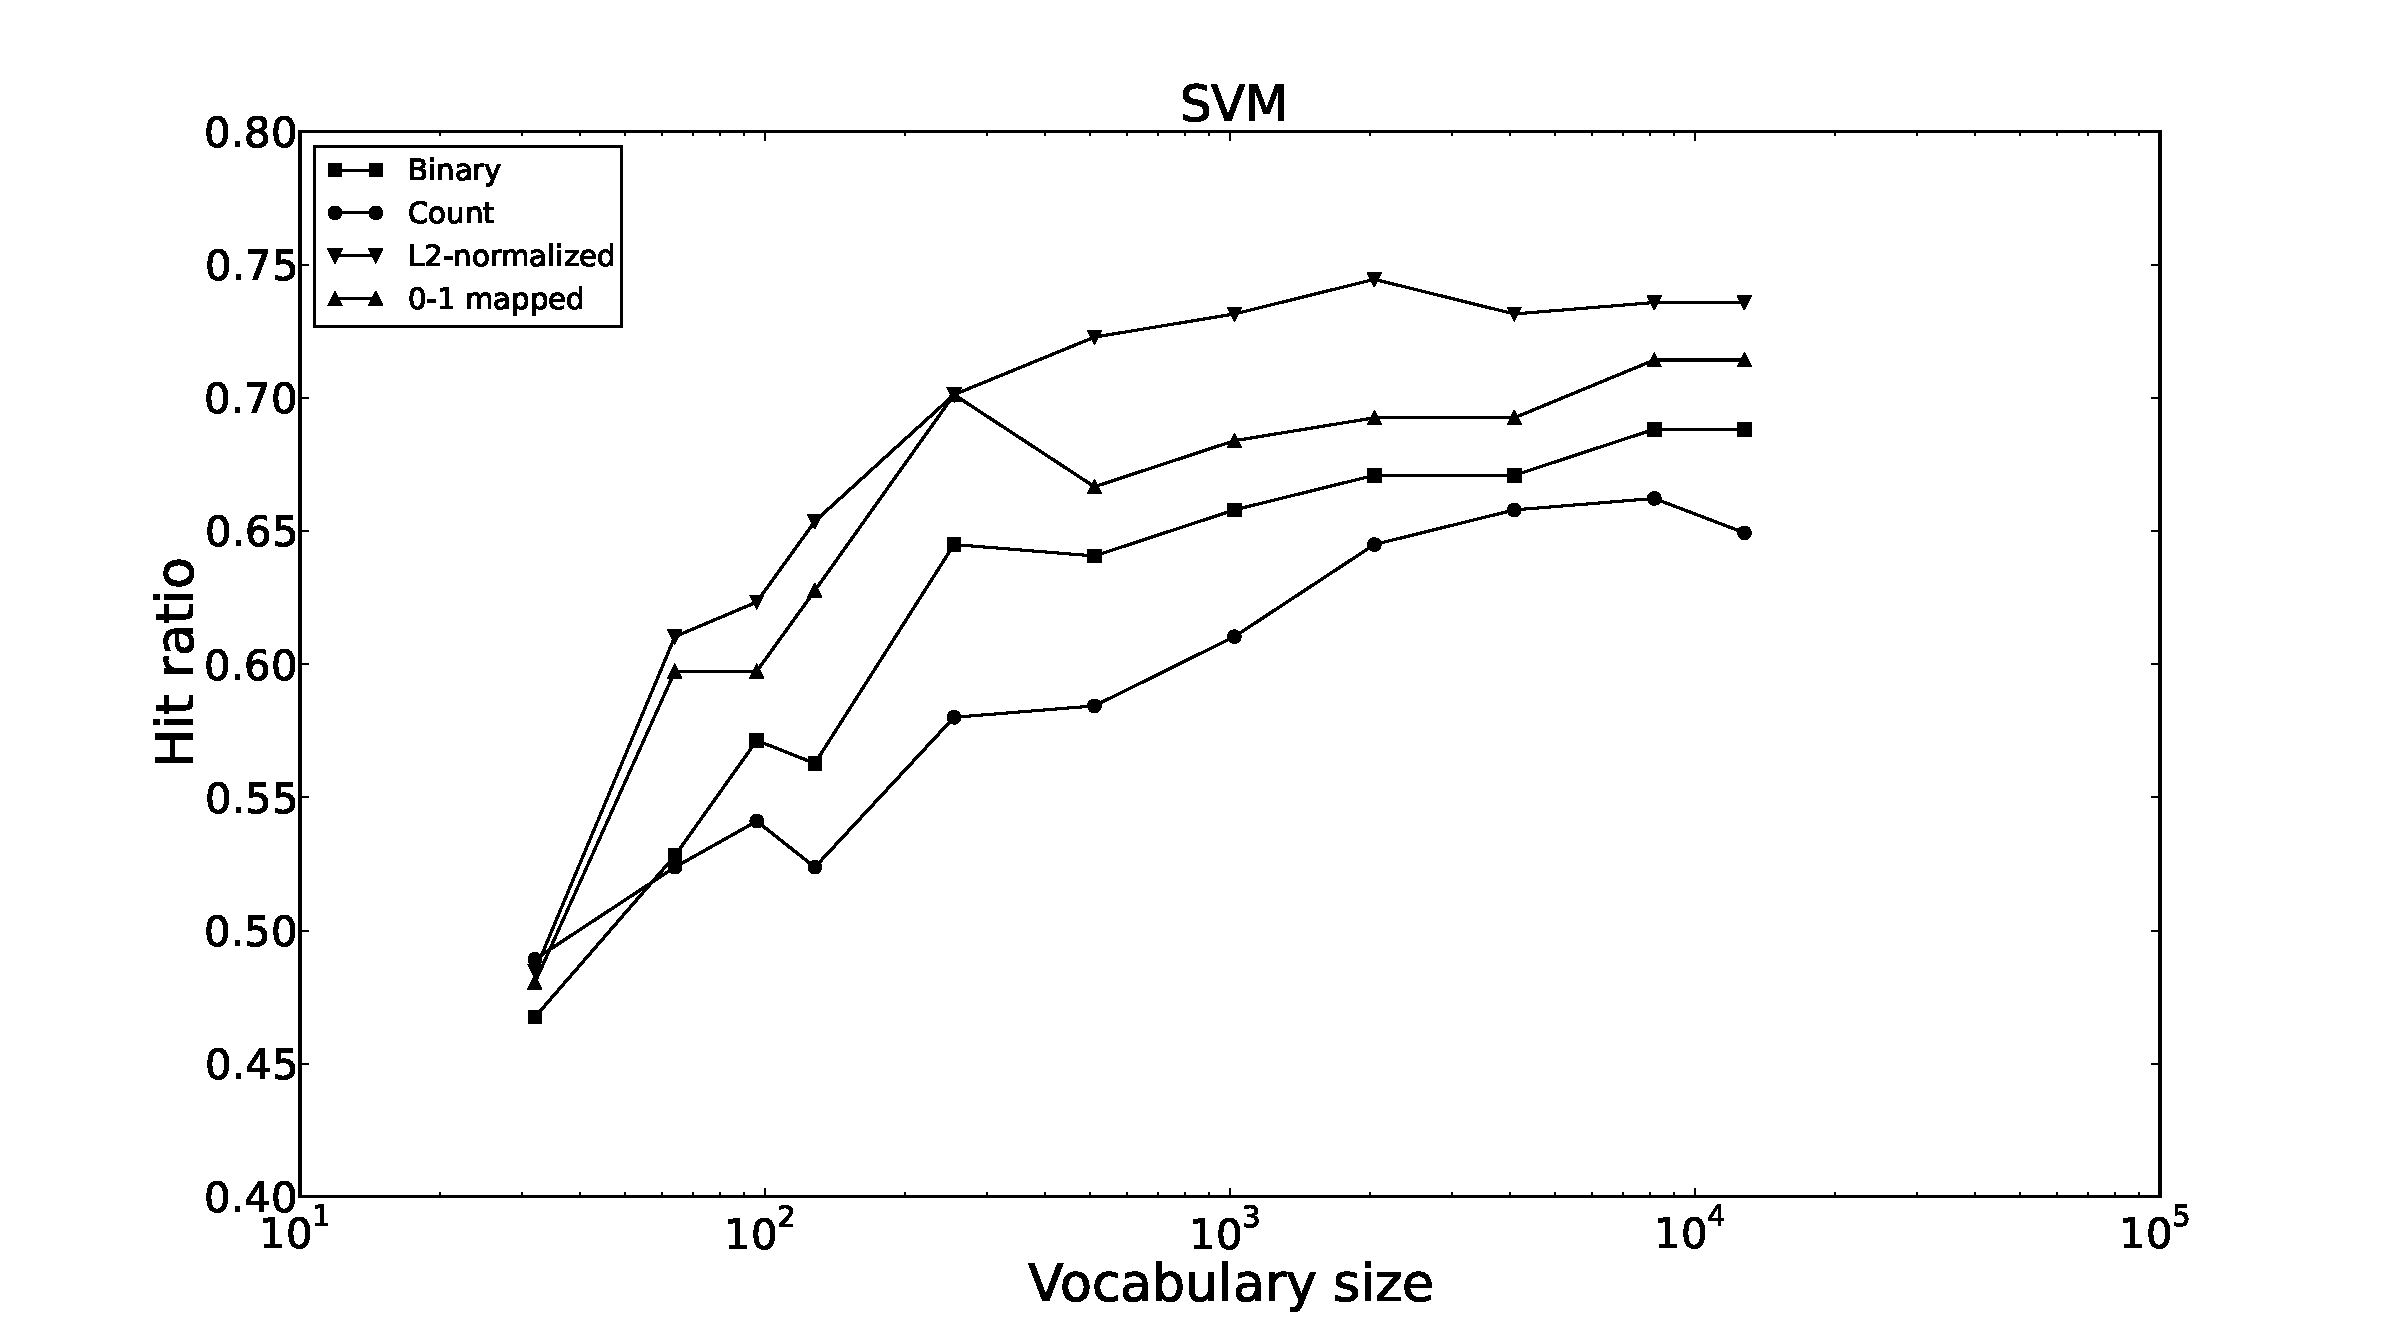
\includegraphics[width=\textwidth]{img/SVM-hitrate-eps-converted-to.pdf}
		\caption{Hit ratio of SVM classifier with varying vocabulary size.}
		\label{fig:hitratio-svm}
	\end{subfigure}
	\\
	\begin{subfigure}[b]{\figwidth}
		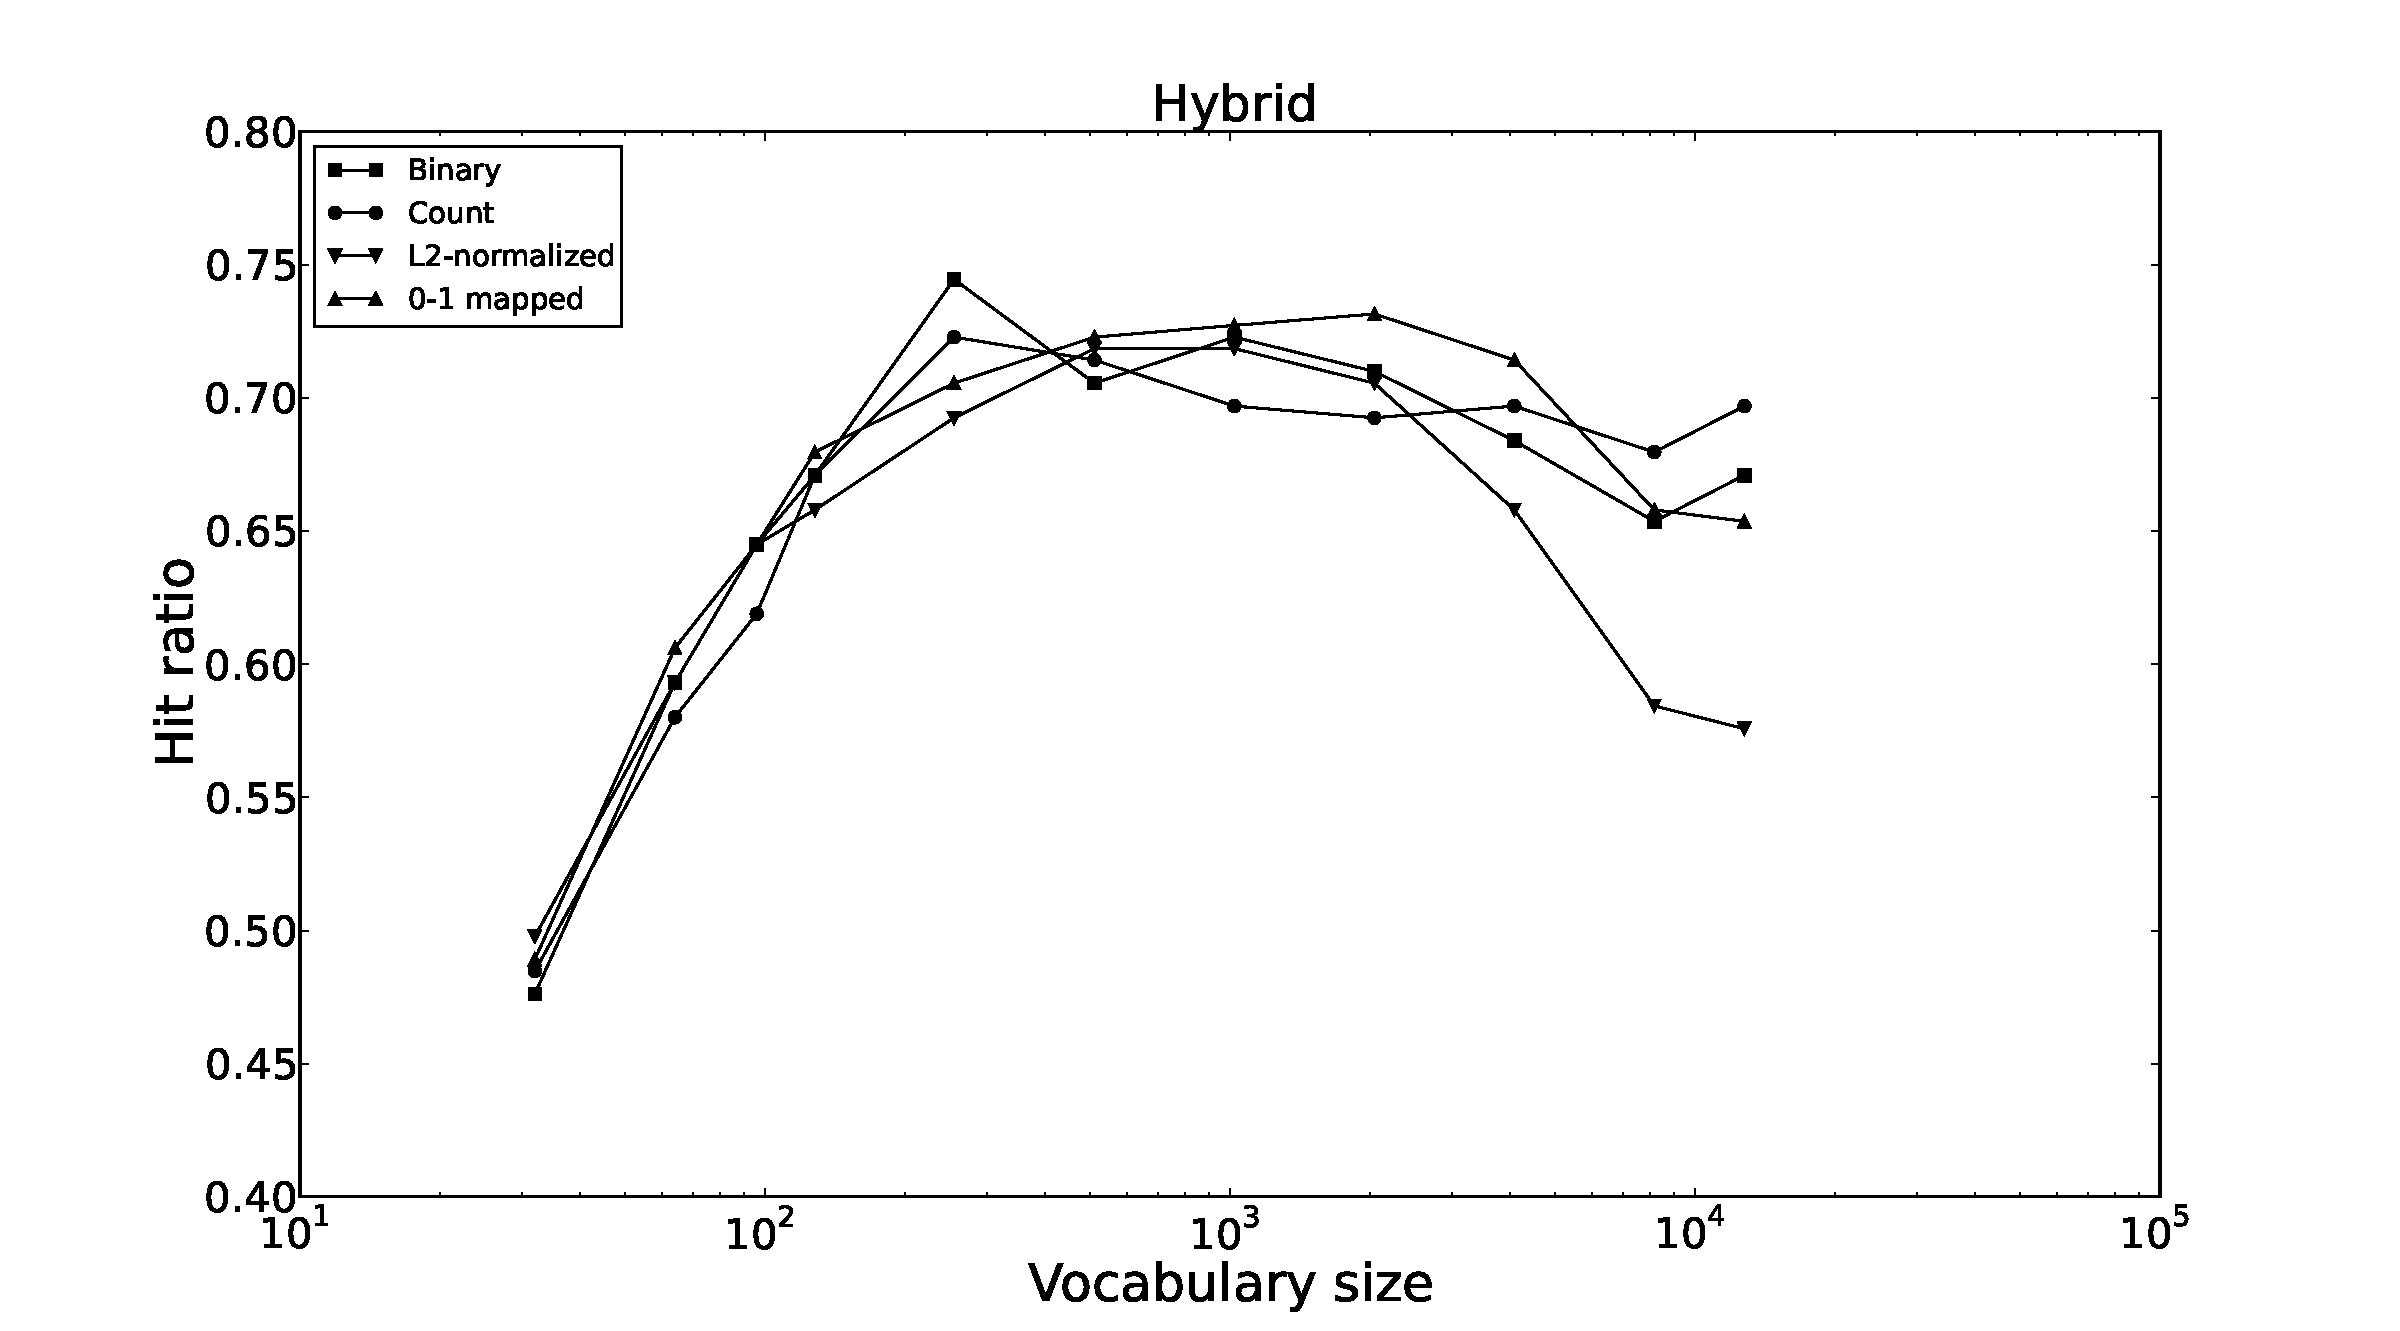
\includegraphics[width=\textwidth]{img/Hybrid-hitrate-eps-converted-to.pdf}
		\caption{Hit ratio of Hybrid classifier with varying vocabulary size.}
		\label{fig:hitratio-hybrid}
	\end{subfigure}
	\caption{Hit ratio vs vocabulary size}
	\label{fig:hitratio}
\end{figure}


\onecolumn
\subsection{Confusion Matrix}
\renewcommand{\figwidth}{0.43\textwidth}
\begin{figure}[H]
	\centering
	\begin{subfigure}[b]{\figwidth}
		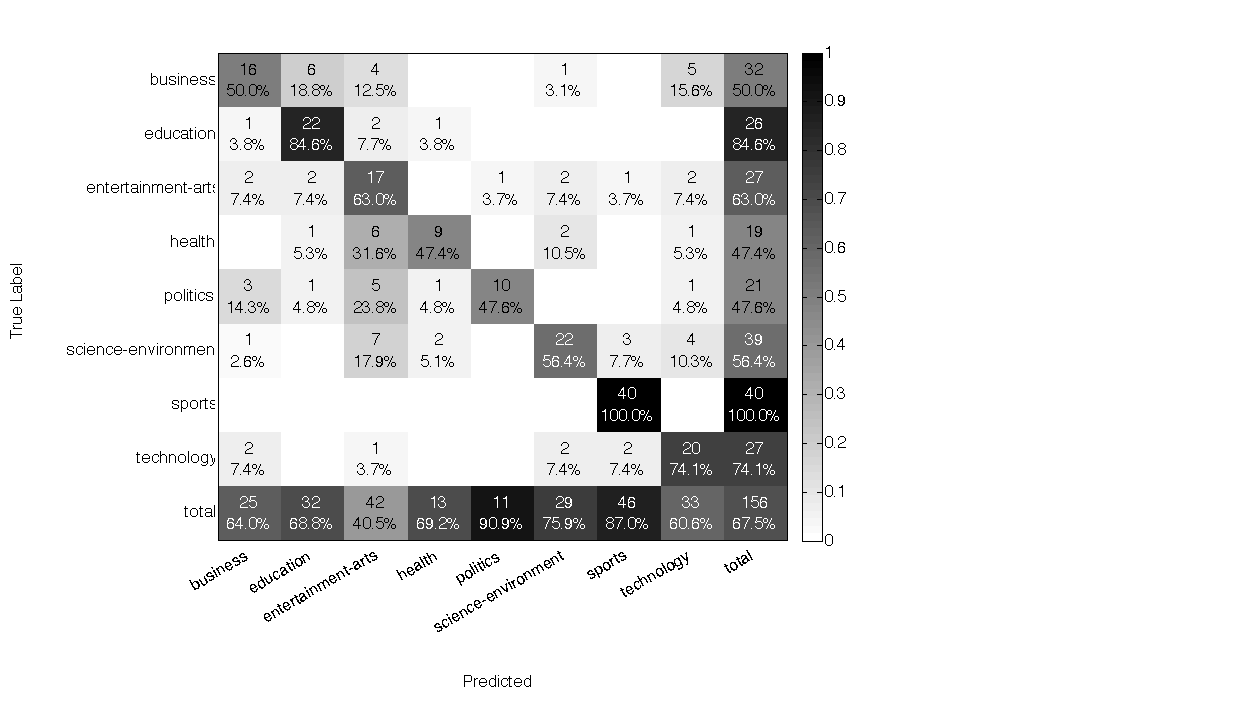
\includegraphics[width=\textwidth,trim=0 0 350 0, clip]{img/Bernou_percentile_5_count.png}
		\caption{Confusion matrix of Bernoulli.}
		\label{fig:confmat-be}
	\end{subfigure}
	~
	\begin{subfigure}[b]{\figwidth}
		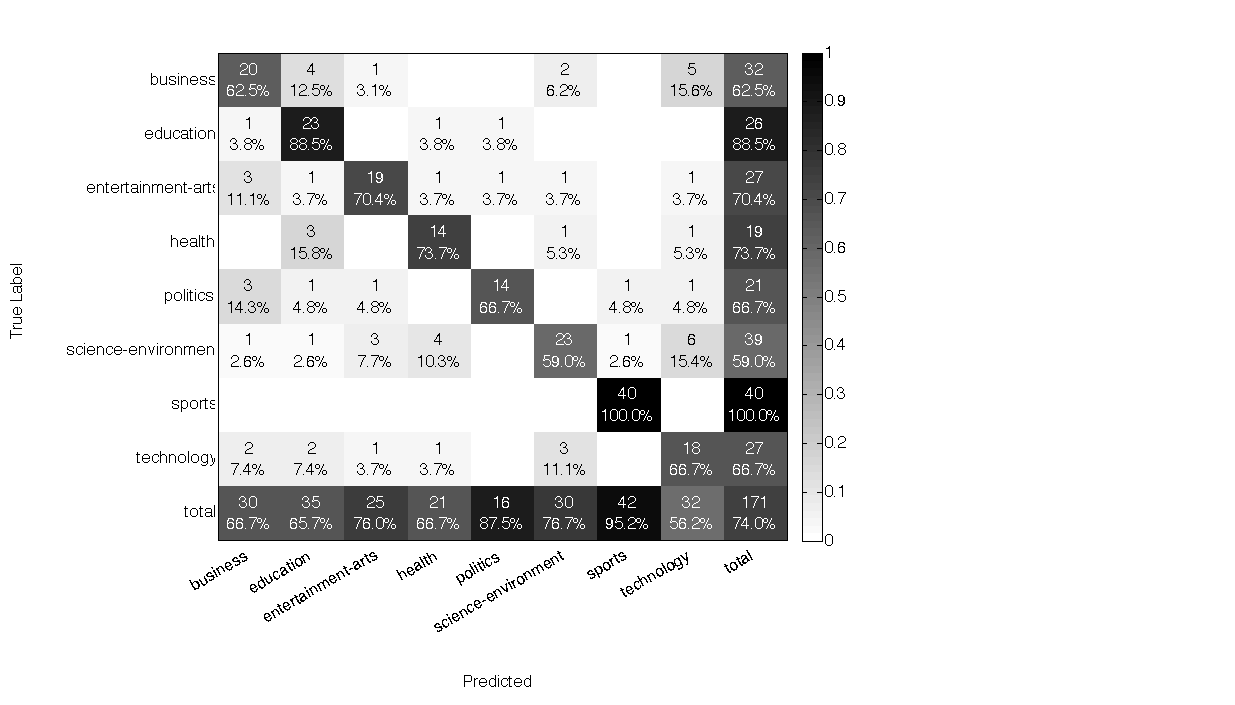
\includegraphics[width=\textwidth,trim=0 0 350 0, clip]{img/Multinomial_percentile_5_count.png}
		\caption{Confusion matrix of Multinomial.}
		\label{fig:confmat-mn}
	\end{subfigure}
	\\
	\begin{subfigure}[b]{\figwidth}
		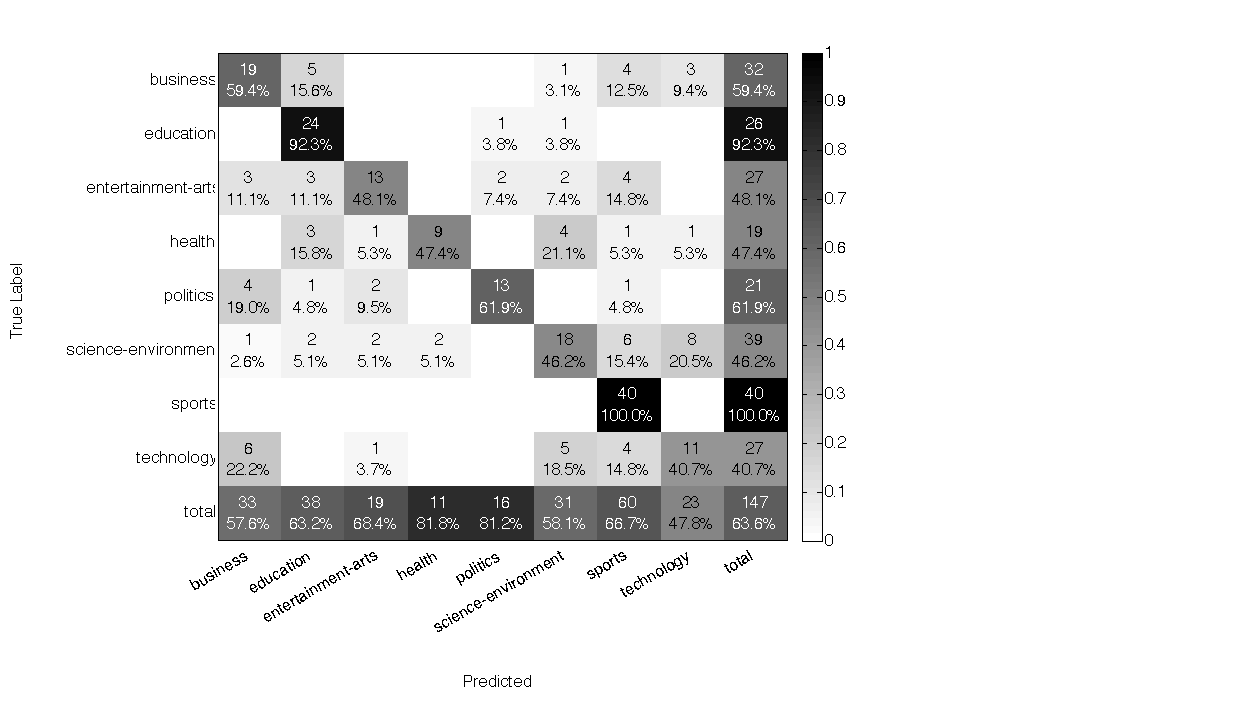
\includegraphics[width=\textwidth,trim=0 0 350 0, clip]{img/RandomForest_percentile_5_count.png}
		\caption{Confusion matrix of Random Forest.}
		\label{fig:confmat-rf}
	\end{subfigure}
	~
	\begin{subfigure}[b]{\figwidth}
		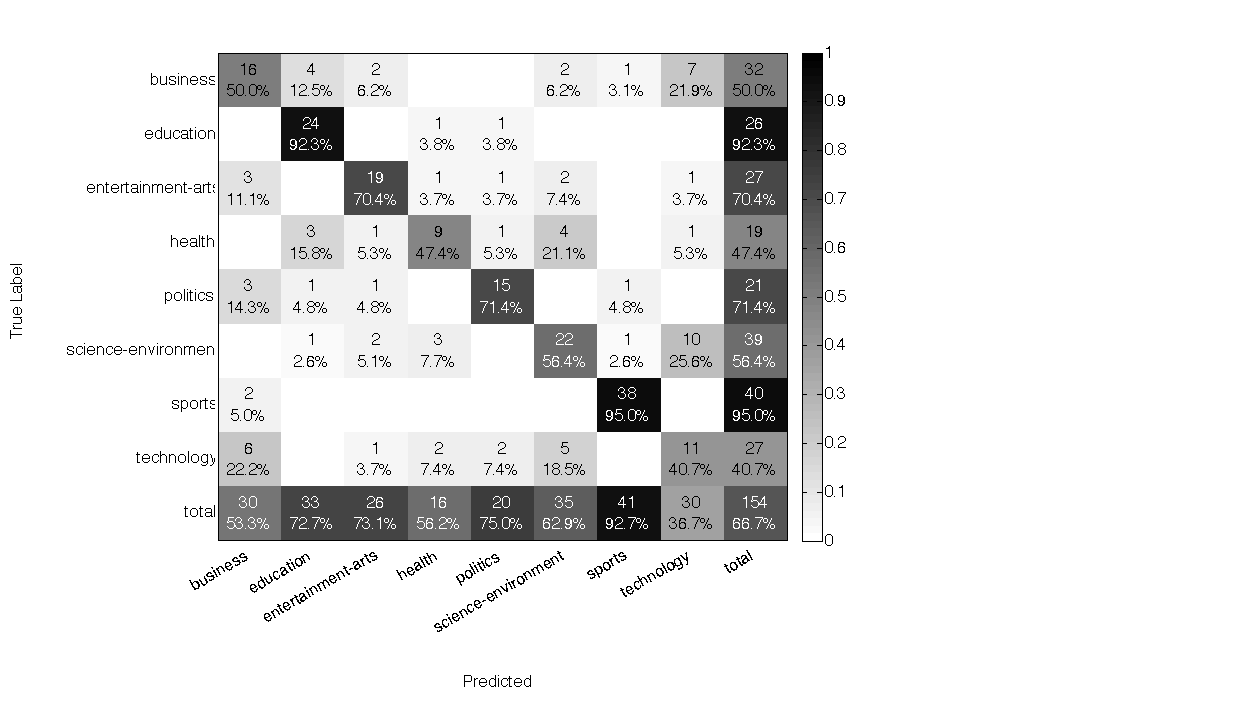
\includegraphics[width=\textwidth,trim=0 0 350 0, clip]{img/SVM_percentile_5_count.png}
		\caption{Confusion matrix of SVM.}
		\label{fig:confmat-svm}
	\end{subfigure}
	\\
	\begin{subfigure}[b]{\figwidth}
		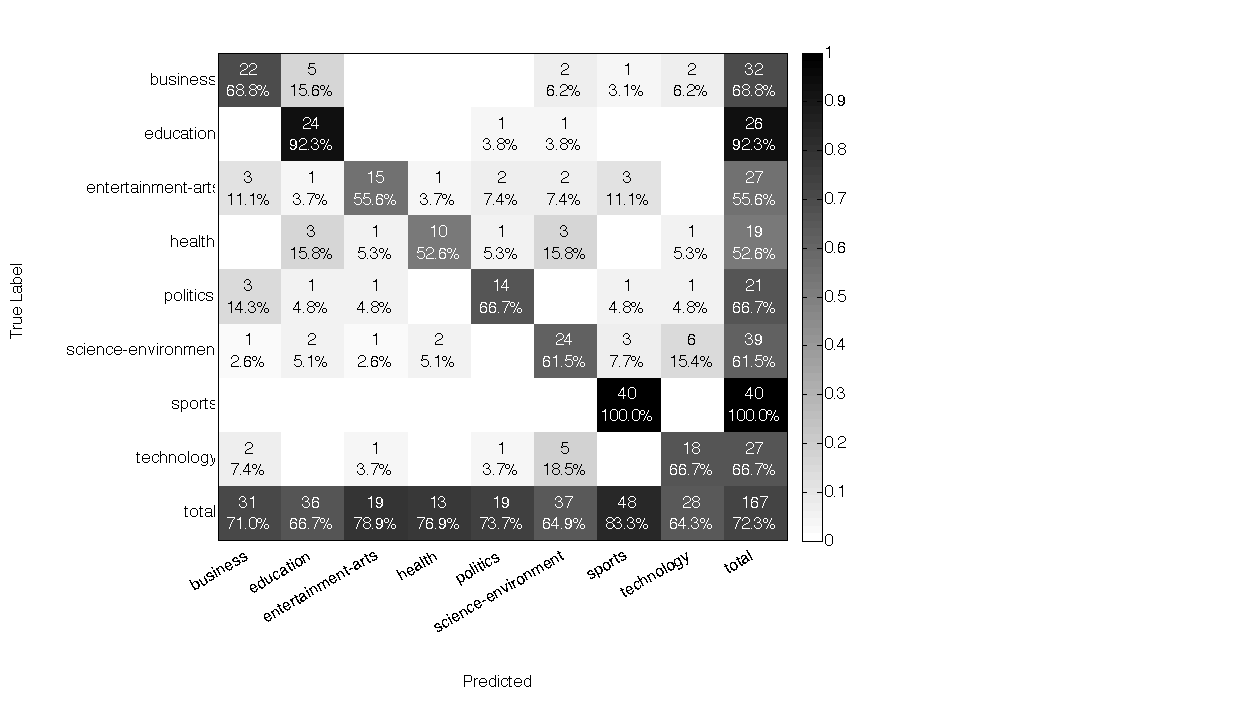
\includegraphics[width=\textwidth,trim=0 0 350 0, clip]{img/hybrid_percentile_5_count.png}
		\caption{Confusion matrix of Hybrid.}
		\label{fig:confmat-hybrid}
	\end{subfigure}
	\caption{Confusion matrices for the different classifiers. A total of 231 articles were tested. A vocabulary size of 511 words and the data type \emph{"Mapped value form 0 to 1"} were used.}
	\label{fig:confmat}
\end{figure}

\twocolumn
\subsection{Similarities}
\begin{table}[h]\footnotesize
	\caption{Percentage that two classifiers, when both classifying wrong, classifies test to the same class. A total of 231 articles were tested. A vocabulary size of 511 words and the data type \emph{"Mapped value from 0 to 1"} was used.}
	\begin{tabular}{r|cccc}
	\ 		 	& Bernoulli & Multin. 	&RF 		&SVM \\ \hline
	Bernoulli 	&100\%   	&67.3\%   	&69.0\%   	&58.8\%\\
	Multin. 	&67.3\%  	&100\%   	&78.6\%   	&76.9\%\\
	RF 			&69.0\%   	&78.6\%  	&100\%   	&75.4\%\\
	SVM 		&58.8\%   	&76.9\%   	&75.4\%  	&100\%
	\end{tabular}
	\label{tab:similarity}
\end{table}